% Created 2013-10-09 Wed 07:07
\documentclass[bigger]{beamer}
\usepackage[utf8]{inputenc}
\usepackage[T1]{fontenc}
\usepackage{fixltx2e}
\usepackage{graphicx}
\usepackage{longtable}
\usepackage{float}
\usepackage{wrapfig}
\usepackage{rotating}
\usepackage[normalem]{ulem}
\usepackage{amsmath}
\usepackage{textcomp}
\usepackage{marvosym}
\usepackage{wasysym}
\usepackage{amssymb}
\usepackage{hyperref}
\tolerance=1000
\usetheme{Madrid}
\author{Aditya Siram}
\date{\today}
\title{Emacsmorgasbord}
\hypersetup{
  pdfkeywords={emacs},
  pdfsubject={A tour of Emacs},
  pdfcreator={Emacs 24.3.50.1 (Org mode 8.2)}}
\begin{document}

\maketitle
\begin{frame}{Outline}
\tableofcontents
\end{frame}


\section{Overview}
\label{sec-1}
\begin{frame}[label=sec-1-1]{What is it?}
\begin{itemize}
\item A text editor
\item 40 years old (70's)
\begin{itemize}
\item In human terms \textasciitilde{}3600 BC
\end{itemize}
\item Steady growth
\item New renaissance b/c scripting languages
\end{itemize}
\end{frame}

\begin{frame}[label=sec-1-2]{Relevance}
\begin{itemize}
\item Hundreds of add-ons
\item Lots of batteries included
\item Works everywhere
\item Very well supported
\begin{itemize}
\item \#emacs
\item gnu.help.emacs
\end{itemize}
\end{itemize}
\end{frame}

\section{Talk Description}
\label{sec-2}
\begin{frame}[label=sec-2-1]{This talk ..}
\begin{itemize}
\item Not flame-bait
\begin{itemize}
\item Also covers Emacs' faults
\end{itemize}
\item No knowledge required
\item Developer biased (because I am one)
\item But also applicable to sysadmins
\item Linux biased
\end{itemize}
\end{frame}

\begin{frame}[label=sec-2-2]{This talk \ldots{}}
\begin{itemize}
\item A whirlwind tour
\item No explanations of every keyboard shortcut
\item Yes, advanced material!
\item Not going for complete understanding
\item Defocus, magic-eye
\item Please ask questions!
\end{itemize}
\end{frame}

\section{Basics}
\label{sec-3}
\begin{frame}[label=sec-3-1]{Terminology}
\begin{columns}
\begin{column}{0.6\textwidth}
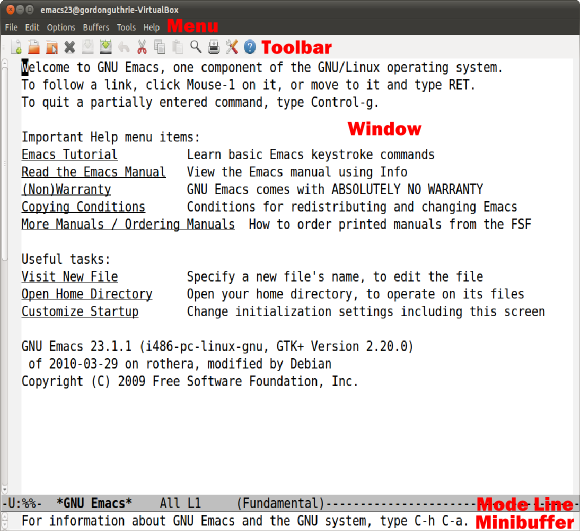
\includegraphics[width=.9\linewidth]{emacs-components.png}
\begin{itemize}
\item `Window` == `buffer`
\item The whole thing is a `frame`
\end{itemize}

\end{column}
\end{columns}
\end{frame}

\begin{frame}[label=sec-3-2]{Lifesavers}
\begin{itemize}
\item `Control-g` or `Esc` - quit whatever I'm doing
\item `C-/` - undo and \uline{3} other keybindings + 'Edit -> Undo'
\end{itemize}
\end{frame}

\begin{frame}[fragile,label=sec-3-3]{Minibuffer}
 \begin{itemize}
\item Invoke with `M-x`
\item `M` \texttt{= "Meta" =} `Alt`
\item All your commands go here
\item `M-x find-file` opens a (new) file
\end{itemize}
\end{frame}

\begin{frame}[label=sec-3-4]{Self-help}
\begin{itemize}
\item `M-x describe-function` - view docs and \uline{keyboard shortcuts}
\item `M-x describe-key` - what function does a shortcut invoke
\item `M-x describe-variable` - view docs and \uline{current value}
\item `M-x info` - general Help facility
\end{itemize}
\end{frame}

\begin{frame}[label=sec-3-5]{Revisit Find-File}
\begin{itemize}
\item `M-x describe-function find-file`
\end{itemize}
\end{frame}

\begin{frame}[label=sec-3-6]{Self-help using Menu Example}
\begin{itemize}
\item View docs on `Insert File`
\item `M-x describe-key C-x i`
\end{itemize}
\end{frame}

\begin{frame}[label=sec-3-7]{Self-help with Toolbar}
\begin{itemize}
\item Requires slightly more experience
\item Know it's called a "toolbar"
\item Probably a map somewhere
\item Probably stored in a variable
\item Try `M-x describe-variable`
\item Also works with `minibuffer`
\end{itemize}
\end{frame}

\begin{frame}[label=sec-3-8]{Structured self-help}
\begin{itemize}
\item `M-x info`
\end{itemize}
\end{frame}

\section{Undoing Changes}
\label{sec-4}
\begin{frame}[label=sec-4-1]{Undo}
\begin{itemize}
\item State is never lost
\item `Redoing` is undoing an undo
\item Yes, it's confusing
\end{itemize}
\end{frame}

\begin{frame}[label=sec-4-2]{Undo-Tree}
\begin{itemize}
\item Visualize changes in a tree
\item Go back to any point
\item Timestamp changes
\item Diff mode
\end{itemize}
\end{frame}

\section{Cut/Copy/Paste}
\label{sec-5}
\begin{frame}[label=sec-5-1]{Cutting/Copying}
\begin{itemize}
\item All cuts and copy's are saved to the `kill-ring`
\item `C-y` pastes the most recent thing
\item `M-y` goes back in history
\item `M-x describe-variable kill-ring` - view the kill-ring
\end{itemize}
\end{frame}

\begin{frame}[label=sec-5-2]{Rectangle Mode}
\begin{itemize}
\item Select/delete/paste rectangular blobs of text
\item Good for column based editing
\item `ps -aux` example
\begin{itemize}
\item keep only root processes with pids
\end{itemize}
\item Can't go past EOL
\begin{itemize}
\item Vim's Visual block is much better
\end{itemize}
\item `df -h` example
\begin{itemize}
\item Move mount points before the usage
\end{itemize}
\end{itemize}
\end{frame}

\begin{frame}[label=sec-5-3]{Picture mode}
\begin{itemize}
\item Drawing ASCII diagrams
\item Fixes all the issues with rectangle-mode
\item Can select arbitrary regions
\end{itemize}
\end{frame}

\section{Working with code}
\label{sec-6}
\begin{frame}[label=sec-6-1]{Occur-mode}
\begin{itemize}
\item Match and \uline{edit} lines that match regex
\end{itemize}
\end{frame}

\begin{frame}[label=sec-6-2]{Imenu}
\begin{itemize}
\item python example
\end{itemize}
\end{frame}

\section{Org Mode}
\label{sec-7}
\begin{frame}[label=sec-7-1]{Org-beamer}
\begin{itemize}
\item this talk
\end{itemize}
\end{frame}

\begin{frame}[label=sec-7-2]{Org-babel}
\begin{itemize}
\item Show code file
\end{itemize}
\end{frame}

\begin{frame}[label=sec-7-3]{Org-table}
\begin{itemize}
\item Simple Table
\item Df revisited
\end{itemize}
\end{frame}

\section{References}
\label{sec-8}
\begin{frame}[label=sec-8-1]{References}
\begin{itemize}
\item \url{http://learn-elisp-for-emacs.org}
\end{itemize}
\end{frame}
% Emacs 24.3.50.1 (Org mode 8.2)
\end{document}
